\chapter{適用例}\label{cha:Indication}
本章では、適用例を用いて、今回試作した\toolName が正しく動作することを確認する。
\toolName が変更前のWebページのURLと、変更後のWebページのURLを入力として、
以下に示す8つのPNG形式の画像を生成する。
\begin{itemize}
    \item Webページの変更前画像
    \item Webページの変更後画像
    \item 画像比較に基づく差分箇所を、色付きの枠で囲むことで強調表示した、Webページの変更前画像
    \item 画像比較に基づく差分箇所を、色付きの枠で囲むことで強調表示した、Webページの変更後画像
    \item HTMLコードの変更に基づく変更箇所を、色付きの枠で囲むことで強調表示した、Webページの変更前画像
    \item HTMLコードの変更に基づく変更箇所を、色付きの枠で囲むことで強調表示した、Webページの変更後画像
    \item レイアウトの不具合箇所を、色付きの枠で囲むことで強調表示した、Webページの変更前画像
    \item レイアウトの不具合箇所を、色付きの枠で囲むことで強調表示した、Webページの変更後画像
\end{itemize}
今回の検証を行うために、以下のWebページを用意する。
\begin{itemize}
    \setlength{\itemsep}{0pt}
          \setlength{\parsep}{0pt}
    \item テスト対象とするWebページA\label{item: ex1_bf}
    \item AのWebページに対して、レイアウトの不具合が発生する変更を埋め込んだWebページB\label{item: ex1_af}
\end{itemize}
テスト対象とするWebページAを図\ref{fig:bf_original}に、
図\ref{fig:bf_original}のWebページAにレイアウトの不具合箇所が発生する変更を埋め込んだWebページBを図\ref{fig:af_original}に、
それぞれ示す。
% 以降、上記の2つのWebページを適用例に用いて、レイアウトの不具合箇所を可視化できることを確認する。

\begin{figure}[htbp]
    \centering
    % 画像ファイル名とサイズを指定
    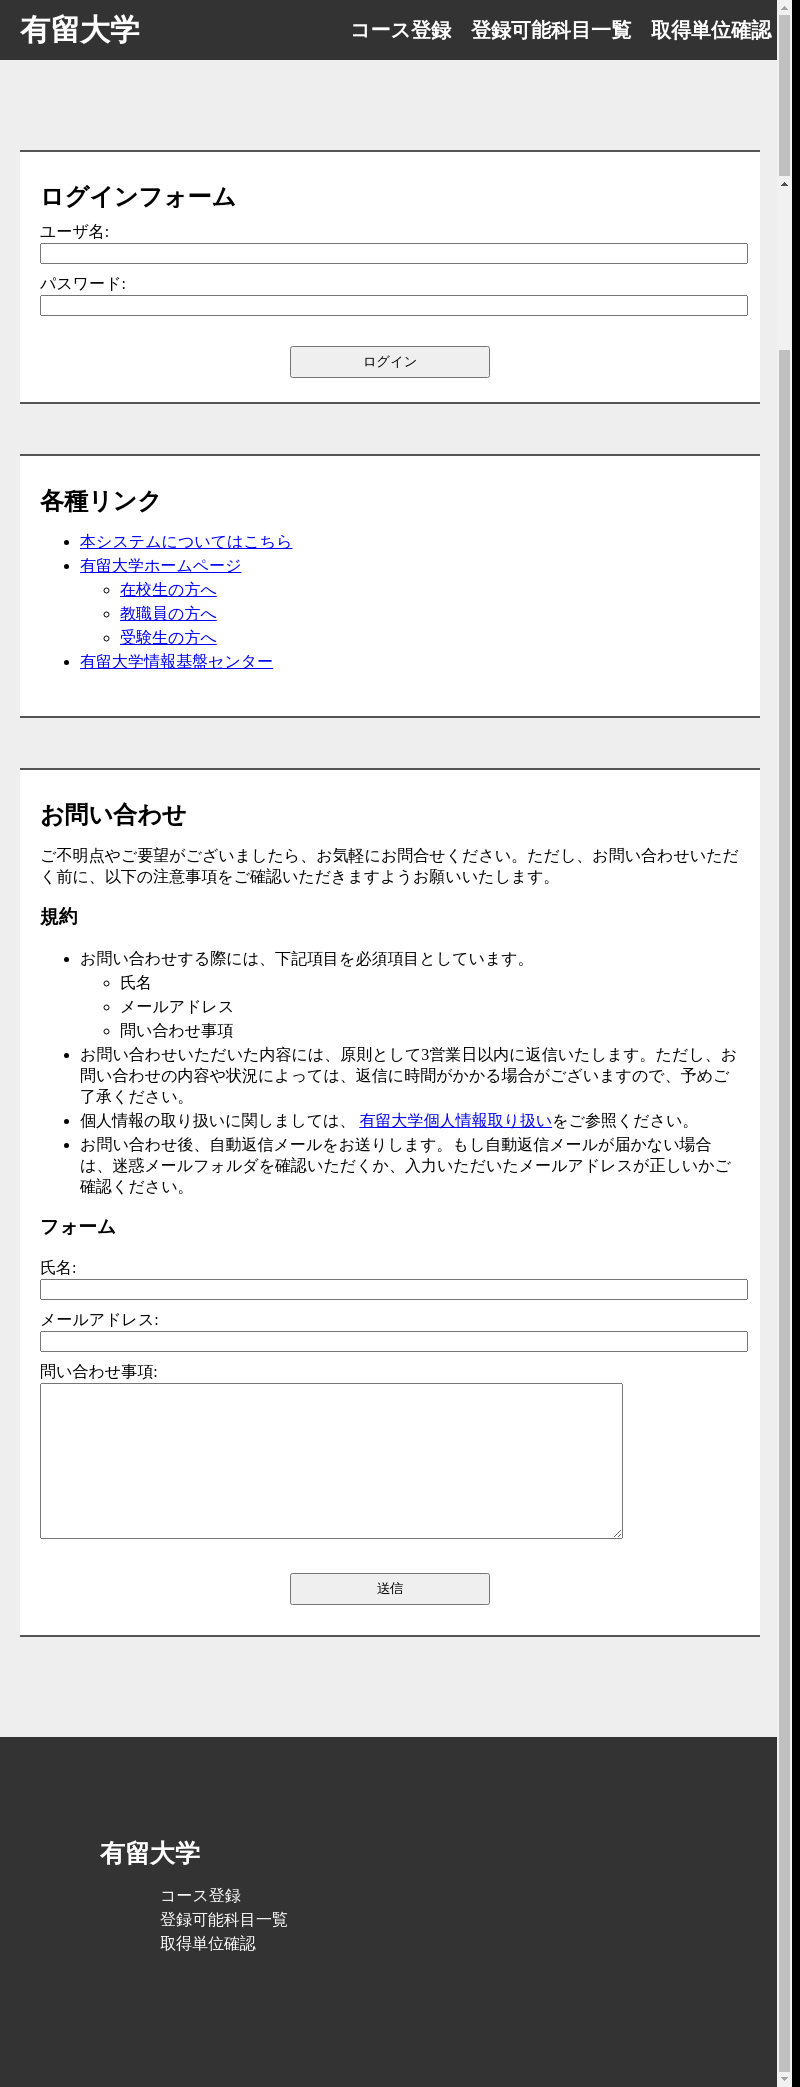
\includegraphics[width=0.5\textwidth]{image/5/original_png/bf_original.png}
    \caption{テスト対象とするWebページA}
    \label{fig:bf_original}
\end{figure}

\begin{figure}[htbp]
    \centering
    % 画像ファイル名とサイズを指定
    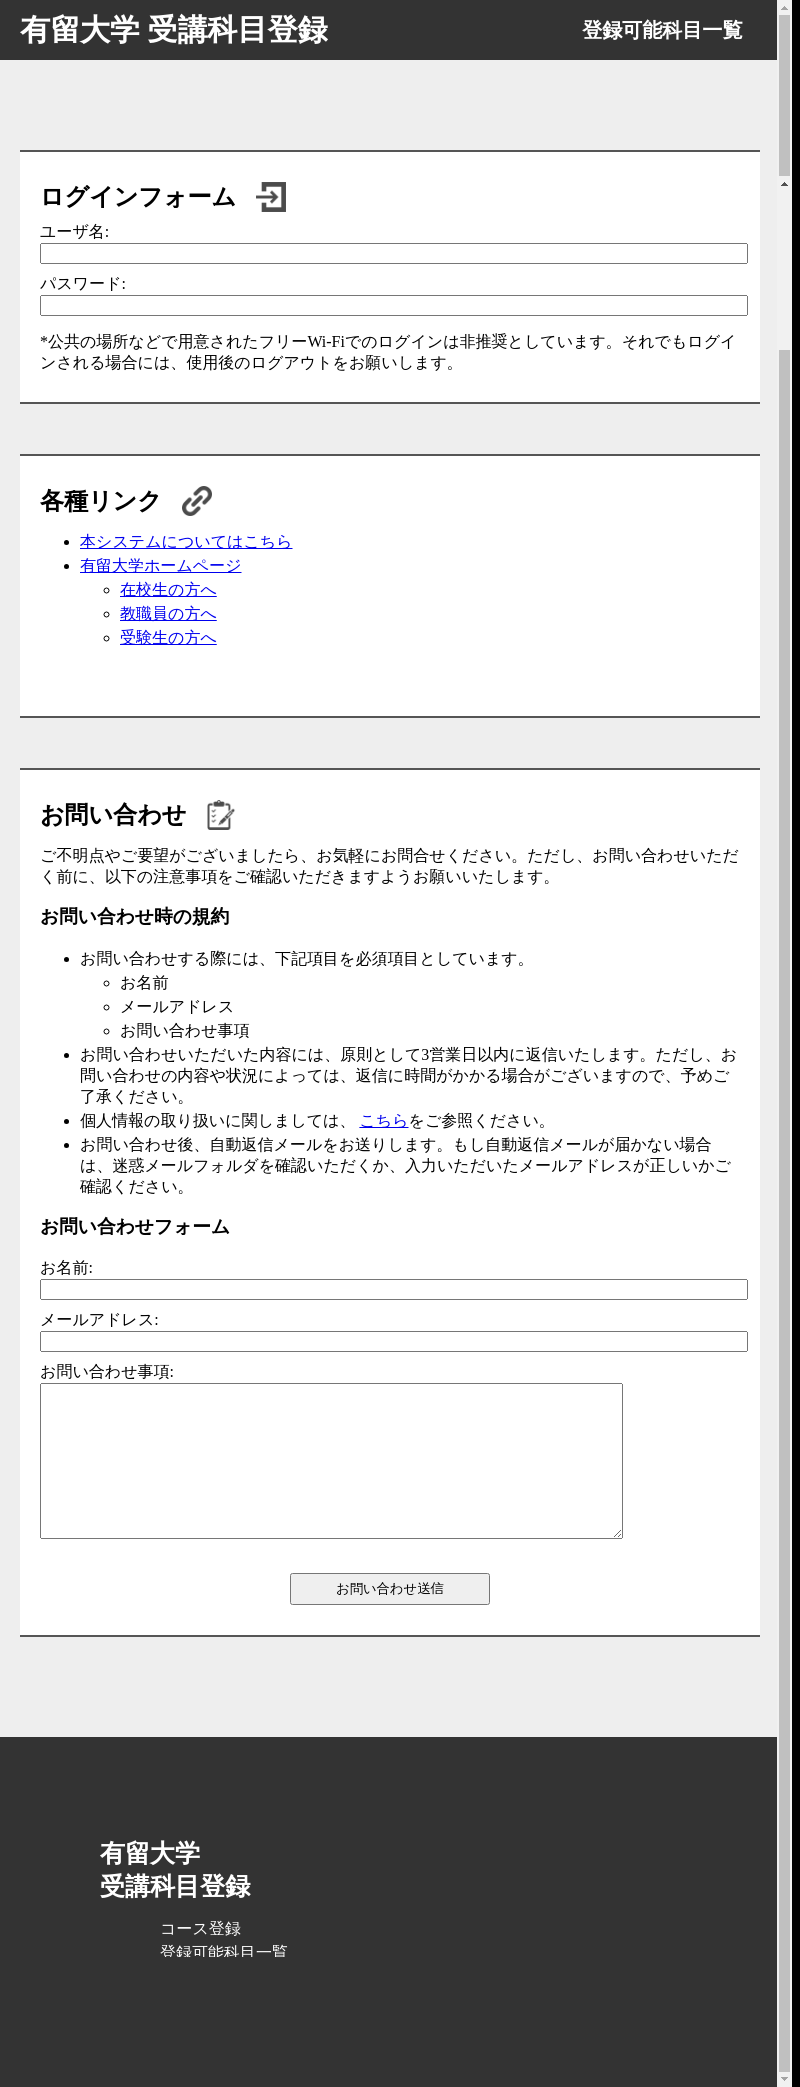
\includegraphics[width=0.5\textwidth]{image/5/original_png/af_original.png}
    \caption{図\ref{fig:bf_original}のWebページAにレイアウトの不具合が発生する変更を埋め込んだWebページB}
    \label{fig:af_original}
\end{figure}
上記のWebページを使用することで、
適用例に対して視覚的回帰テストを行った\toolName の各表示タブを確認することができる。

以降の節では、適用例を用いて、\toolName が持つ以下のそれぞれの機能について、確認する。
% 画像比較に基づく差分箇所表示、HTMLコードの変更に基づく変更箇所表示、レイアウトの不具合箇所表示
% のそれぞれの
% 画像比較に基づく差分箇所からHTMLコードに基づかないレイアウトの不具合箇所を
% 可視化できることを確認する。
% \toolName のUIは、以下に示す4つのタブを持つタブメニューと、各タブに対応するタブコンテンツからなる。
% \begin{itemize}
%     \item[①] タブメニュー
%           \begin{itemize}
%               \item オリジナル表示タブ
%               \item 画像比較に基づく差分箇所表示タブ
%               \item HTMLコードの変更に基づく変更箇所表示タブ
%               \item レイアウトの不具合箇所表示タブ
%           \end{itemize}
%     \item[②] タブコンテンツ
% \end{itemize}
% \par
% \toolName を用いて、HTMLコードに基づかないレイアウトの不具合箇所を可視化できるかどうかを確認するために、以下の4つのパターンについて確認する。
% \begin{itemize}
%     \item  画像比較に基づく差分箇所通りにHTMLコードに基づく変更箇所に削除されている
%     \item 画像比較に基づく差分箇所通りにHTMLコードに基づく変更箇所に削除されていない
%     \item 画像比較に基づく差分箇所通りにHTMLコードに基づく変更箇所に追加されている
%     \item 画像比較に基づく差分箇所通りにHTMLコードに基づく変更箇所に追加されていない
% \end{itemize}
% \par

\section{画像比較に基づく差分箇所表示の確認}
適用例を用いて、画像比較に基づく差分箇所表示が、正しく行われていることを確認する。
図\ref{fig:bf_original}と図\ref{fig:af_original}の適用例における画像の比較に基づく差分箇所表示を、図\ref{fig: 5_app2}に示す。
図\ref{fig: 5_app2}より、画像比較に基づく差分箇所表示が、正しく行われていることを確認できる。

\begin{figure}[tp]
    \begin{center}
        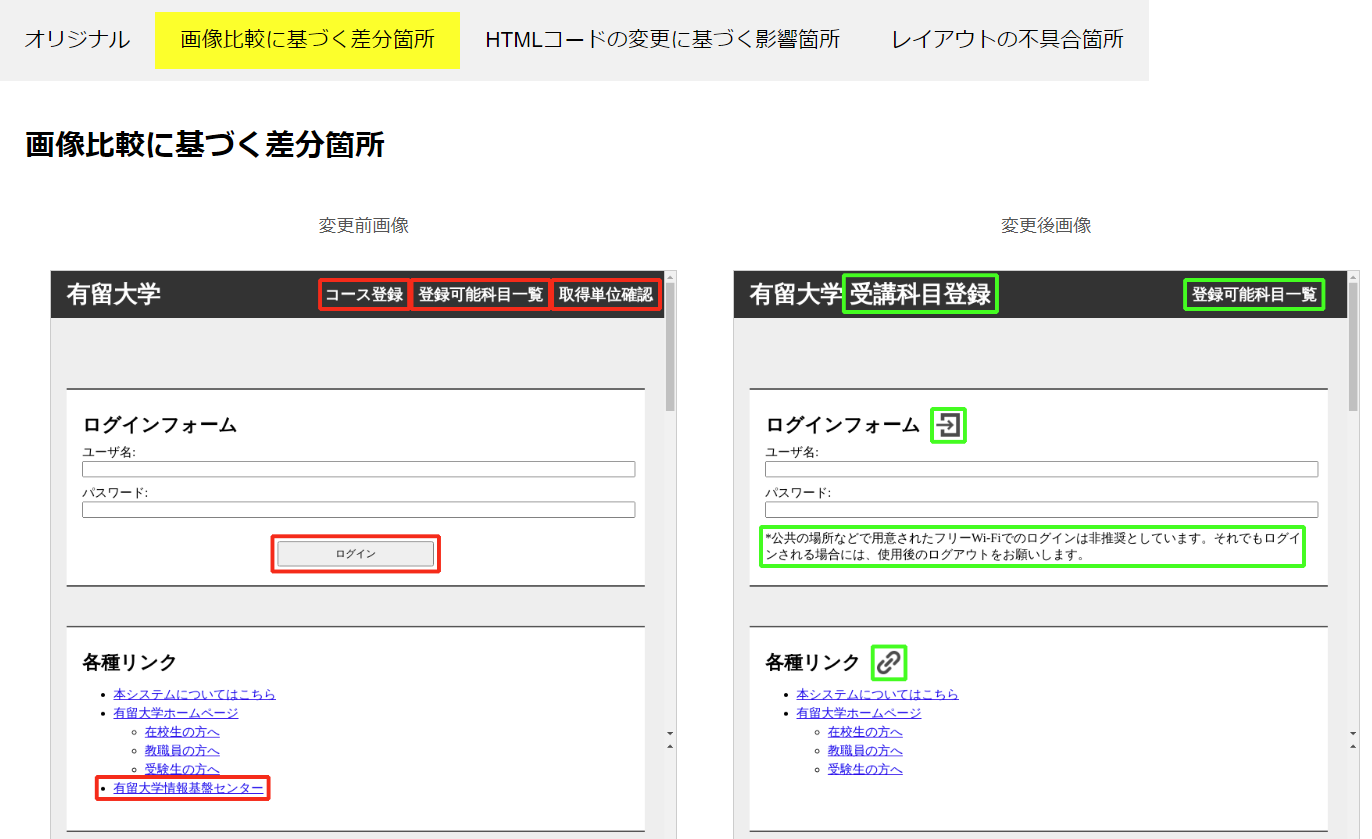
\includegraphics[width=1.0\columnwidth]{image/5/5_app2.png}
        \caption{図\ref{fig:bf_original}と図\ref{fig:af_original}における画像比較に基づく差分箇所表示}
        \label{fig: 5_app2}
    \end{center}
\end{figure}



\section{HTMLコードの変更に基づく変更箇所表示の確認}
適用例を用いて、HTMLコードの比較に基づく変更箇所表示が、正しく行われていることを確認する。
図\ref{fig:bf_original}と図\ref{fig:af_original}の適用例における変更箇所表示を、図\ref{fig: 5_app1}に示す。
図\ref{fig: 5_app1}より、HTMLコードの比較に基づく変更箇所表示が、正しく行われていることを確認できる。
\begin{figure}[tp]
    \begin{center}
        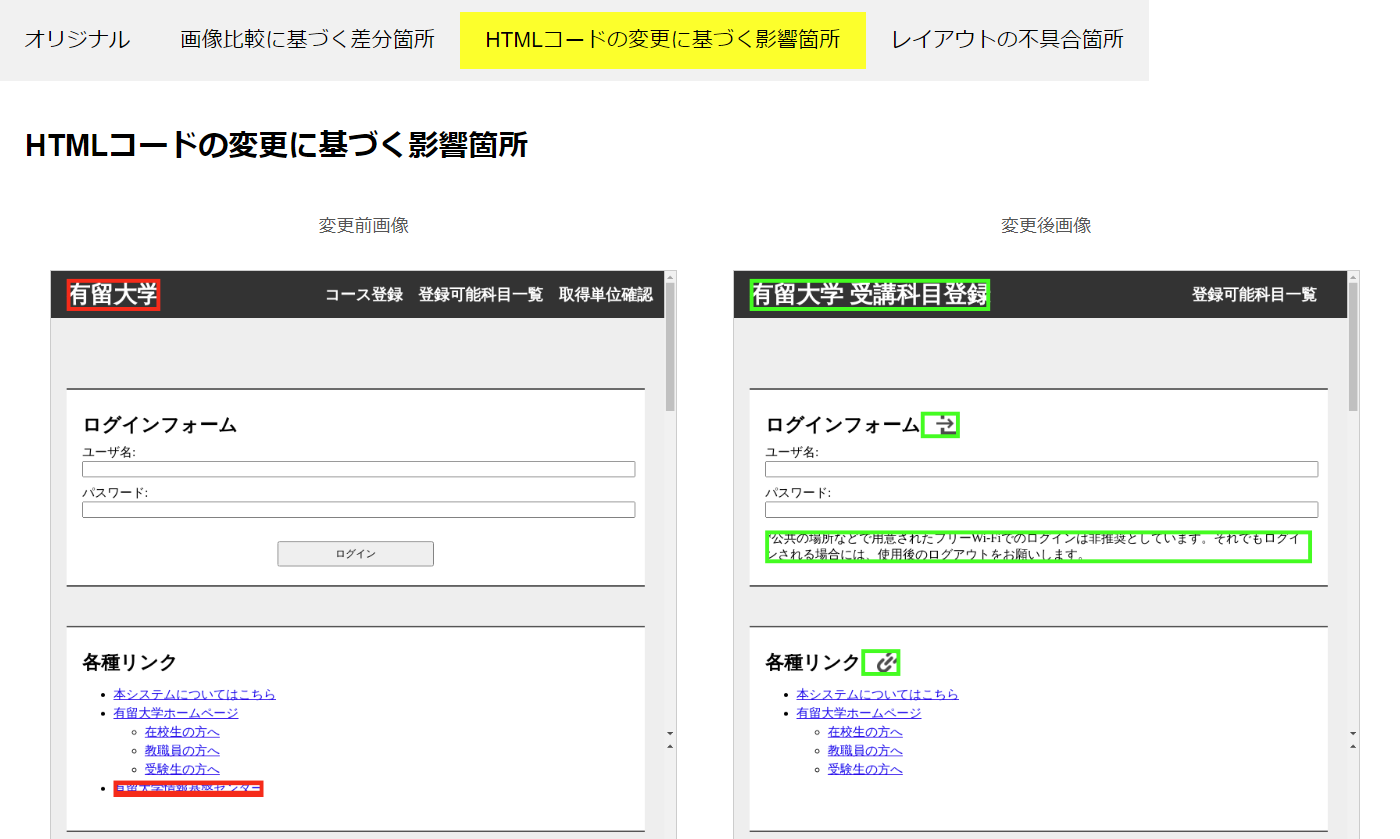
\includegraphics[width=1.0\columnwidth]{image/5/5_app1.png}
        \caption{図\ref{fig:bf_original}と図\ref{fig:af_original}の適用例における変更箇所表示}
        \label{fig: 5_app1}
    \end{center}
\end{figure}


\section{レイアウトの不具合箇所表示の確認}
適用例を用いて、レイアウトの不具合箇所表示が、正しく行われていることを確認する。
図\ref{fig:bf_original}と図\ref{fig:af_original}の適用例におけるレイアウトの不具合箇所表示を、図\ref{fig: 5_app3}に示す。
HTMLコードに基づかないレイアウトの不具合箇所を確認するために、以下の4つのパターンについて確認する。
\begin{itemize}
    \item 画像比較に基づく差分箇所通りにHTMLコードに基づく変更箇所に削除されている
    \item 画像比較に基づく差分箇所通りにHTMLコードに基づく変更箇所に削除されていない
    \item 画像比較に基づく差分箇所通りにHTMLコードに基づく変更箇所に追加されている
    \item 画像比較に基づく差分箇所通りにHTMLコードに基づく変更箇所に追加されていない
\end{itemize}
図\ref{fig: 5_app3}より、レイアウトの不具合箇所表示が、正しく行われていることを確認できる。
\begin{figure}[tp]
    \begin{center}
        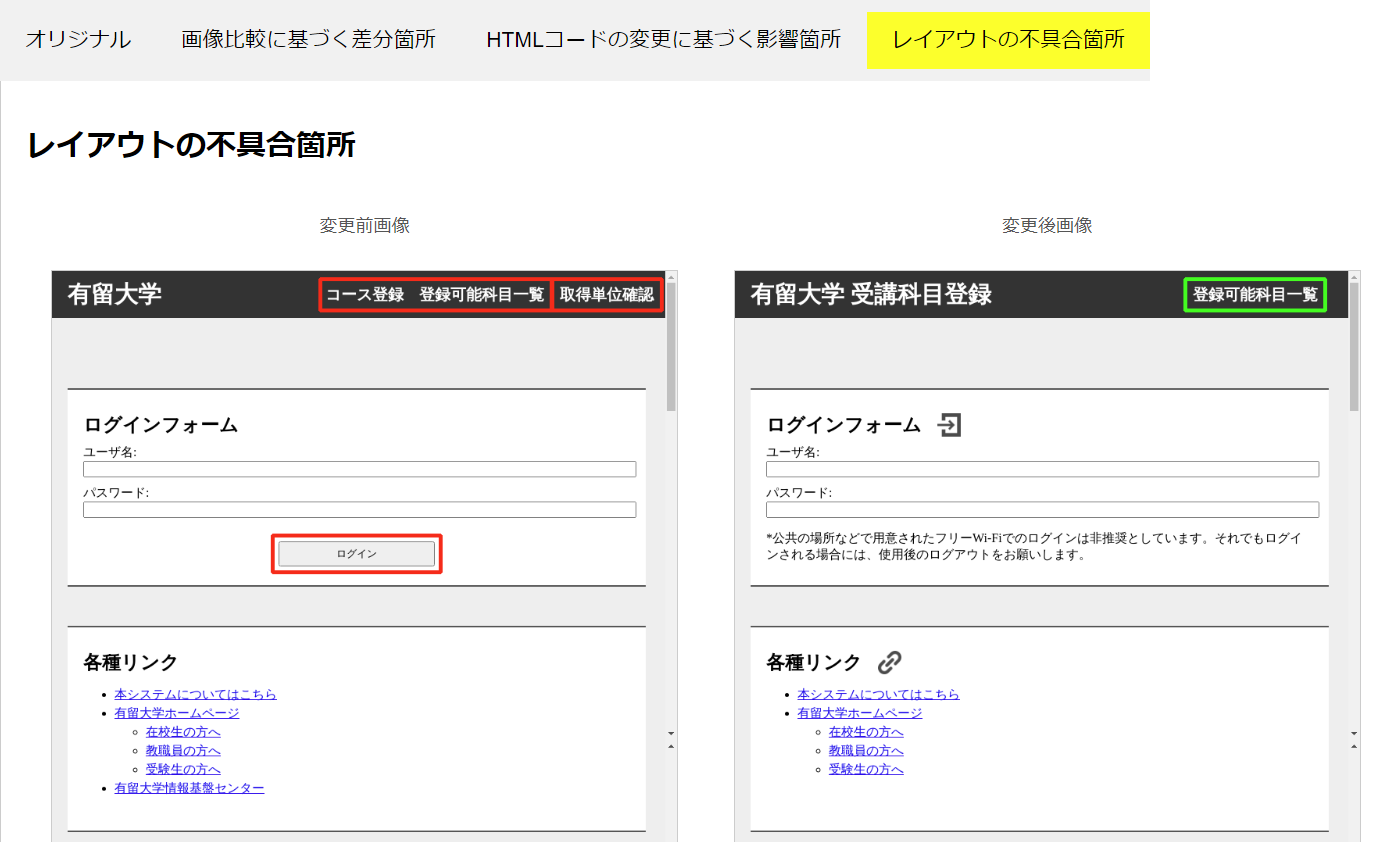
\includegraphics[width=1.0\columnwidth]{image/5/5_app_3.png}
        \caption{図\ref{fig:bf_original}と図\ref{fig:af_original}の適用例におけるレイアウトの不具合箇所表示}
        \label{fig: 5_app3}
    \end{center}
\end{figure}




\subsection{パターン1: 差分箇所通りに削除されている}\label{sec:result_area_detection}
適用例を用いて、差分箇所通りに削除されていることを確認する。
図\ref{fig: 5_app2}の画面を確認すると、変更前画像上の一番下のリンクが赤枠で囲まれていることが分かる。
この赤枠に着目すると、赤枠は変更後画像上で削除されていることが分かる。
次に、差分箇所通りに削除されているかどうかを確かめるために、
図\ref{fig: 5_app1}のHTMLコードの比較に基づく変更箇所表示タブを確認すると、
赤枠で囲まれているため、HTMLコードに基づいて削除された箇所だと分かる。
最後に、図\ref{fig: 5_app3}のレイアウトの不具合箇所表示タブで確認すると、
レイアウトの不具合箇所として赤枠で囲まれていないことが分かる。
\par
よって、\toolName は、差分箇所通りに削除されていることを確認できる。



\subsection{パターン2: 差分箇所通りに削除されていない}\label{sec:result_area2}
適用例を用いて、差分箇所通りに削除されていないことを確認する。
図\ref{fig: 5_app2}の画面を確認すると、変更前画像上のログインボタンが赤枠で囲まれていることが分かる。
この赤枠に着目すると、変更後画像上で削除されていることが分かる。
次に、差分箇所通りに削除されているかどうかを確かめるために、
図\ref{fig: 5_app1}のHTMLコードの比較に基づく変更箇所表示タブを確認すると、
赤枠で囲まれていないため、HTMLコードに基づいて削除されていない箇所だと分かる。
このことから、緑枠で囲まれたテキストによって、ログインボタンが隠れた状態になっていると推測できる。
最後に、図\ref{fig: 5_app3}のレイアウトの不具合箇所表示タブで確認すると、
レイアウトの不具合箇所として赤枠で囲まれていることが分かる。
\par
よって、\toolName は、差分箇所通りに削除されていないことを確認できた。


\subsection{パターン3: 差分箇所通りに追加されている}\label{sec:result_area3}
適用例を用いて、差分箇所通りに追加されていることを確認する。
図\ref{fig: 5_app2}の画面を確認すると、変更後画像上の左上テキスト「受講科目登録」が緑枠で囲まれていることが分かる。
この緑枠に着目すると、変更前画像上から追加されていることが分かる。
次に、差分箇所通りに追加されているかどうかを確かめるために、
図\ref{fig: 5_app1}のHTMLコードの比較に基づく変更箇所表示タブを確認すると、
緑枠で囲まれているため、HTMLコードに基づいて追加された箇所だと分かる。
最後に、図\ref{fig: 5_app3}のレイアウトの不具合箇所表示タブで確認すると、
レイアウトの不具合箇所として緑枠で囲まれていないことが分かる。
\par
よって、\toolName は、差分箇所通りに追加されていることを確認できた。


\subsection{パターン4: 差分箇所通りに追加されていない}\label{sec:result_area4}
適用例を用いて、差分箇所通りに追加されていないことを確認する。
図\ref{fig: 5_app2}の画面を確認すると、変更後画像上の右上テキスト「登録可能科目一覧」が緑枠で囲まれていることが分かる。
この緑枠に着目すると、緑枠内のテキストと完全一致するテキストが変更前画像上に赤枠で囲まれているため、
変更前画像上から削除され、変更後画像上に新しく追加されていることが分かる。
% つまり、変更後にテキストの配置の変更があったと推測できる。
次に、差分箇所通りに追加されているかどうかを確かめるために、
図\ref{fig: 5_app1}のHTMLコードの比較に基づく変更箇所表示タブを確認すると、
緑枠で囲まれていないため、HTMLコードに基づいて追加されていない箇所だと分かる。
最後に、図\ref{fig: 5_app3}のレイアウトの不具合箇所表示タブで確認すると、
レイアウトの不具合箇所として緑枠で囲まれていることが分かる。
\par
よって、\toolName は、差分箇所通りに削除されていないことを確認できた。
% \section{画面要素の隠れが発生したWebページ}\label{subsec:result_rect_area}
% \subsection{Case1:開発者の意図しないレイアウトの不具合}\label{subsec:result_rect_area}

% \subsection{Case2:開発者が意図して画面要素を消した場合}\label{subsec:result_underline_area}

% \subsection{Case3:開発者が意図せず画面要素を消した場合}\label{subsec:result_underline}


% \section{画面要素の見切れが発生したWebページ}\label{subsec:result_underline_area}
% \subsection{Case1:開発者の意図しないレイアウトの不具合}\label{subsec:result_rect_area}

% \subsection{Case2:開発者が意図して画面要素を消した場合}\label{subsec:result_underline_area}

% \subsection{Case3:開発者が意図せず画面要素を消した場合}\label{subsec:result_underline}

% \section{画面要素の重なりが発生したWebページ}\label{sec:result_area_detection}

% \subsection{Case1:開発者の意図しないレイアウトの不具合}\label{subsec:result_rect_area}

% \subsection{Case2:開発者が意図して画面要素を消した場合}\label{subsec:result_underline_area}

% \subsection{Case3:開発者が意図せず画面要素を消した場合}\label{subsec:result_underline}